\documentclass[10,aspectratio=169]{beamer}
%Author: Abdul Saboor@UDEL 2019
\mode<presentation> 
\pgfmathsetmacro{\TotalTime}{20}  %Sets time duration.
\usepackage{amsmath}
\usepackage{amsfonts}
\usepackage[english]{babel}
\usepackage[latin1]{inputenc}
\usepackage{color}
\usepackage{xcolor}
\usepackage{hyperref}
\usepackage{lipsum}
\usepackage{wrapfig}
\usepackage{verbatim}
\usepackage{listings}
\usepackage{subfigure}
\usepackage{tikz}
\usepackage{blindtext}
\usepackage{./resources/mystyle}
\usetikzlibrary{fadings, shadows, shadings}
\usepackage{circuitikz}
\usepackage{comment}
\usepackage{ifthen}
\usepackage{multicol}
\usepackage{graphicx} % Allows including images
\usepackage{booktabs} % Allows the use of \toprule, \midrule 
\usefonttheme{serif}
% TO CHANGE DEFAULT LINE SPREAD AT ANY POINT IN DOCUMENT
\renewcommand{\baselinestretch}{0.9} 
\author{{\bf Abdul Saboor} \\ {\scriptsize Email: asaboor@udel.edu}} 
\institute[UDEL]
{Department of Physics and Astronomy \\ University of Delaware, Newark, DE 19716-2570, USA} 
\title[]{\href{https://github.com/massgh/Beamer-Timer/tree/master/}{\bf \LARGE{Time Beam  \\ Progress Bar}}}
\date{\tddate\ \ \tdtime}
\begin{document}
%-----------------------------------------------------------------------
%	PRESENTATION SLIDE TITLE
%----------------------------------------------------------------------- 
{
\usebackgroundtemplate{\begin{tikzpicture}
		\node[align=center,opacity=0.2]{ 
\includegraphics[width=0.55\paperwidth]{resources/ud.png}};
	\end{tikzpicture}}
\begin{frame}[plain,noframenumbering]
\begin{center}
	\begin{tikzpicture}	
		\node[text width= 0.3\textwidth, align=center,rounded corners,fill=white,inner sep=0.3ex] 
		 at (0.5*\paperwidth,0) {
\includegraphics[width=\textwidth]{resources/ud1}};
	
		\draw[] node[ text width= 0.75\textwidth ,style=title text] at (0.5*\paperwidth,-4) { \begin{minipage}{\textwidth} 
		\maketitle
		\end{minipage}};
	\end{tikzpicture}
\end{center}
\end{frame}
}
%----------------------------------------------------------------------- 
%SLIDES AFTER TITLE START HERE
%-----------------------------------------------------------------------
%	PRESENTATION SLIDE 1
%----------------------------------------------------------------------- 
\SingleFrame{OutLine}{
	\initclock  % This must be used one time to initialize the clock
	\begin{center}
		\sNode{ \vspace{-6mm}
		\begin{multicols}{2}
			\tableofcontents
		\end{multicols}}
\end{center}
}
%-----------------------------------------------------------------------
%	PRESENTATION SLIDE 2
%----------------------------------------------------------------------- 
\section{Single Column Frame}
\SingleFrame{Single Column Frame}{
\sNode{ A frame with one column accepts two arguments like below: \\
		\alert{$\backslash$SingleFrame\{Frame Title\}\{Frame Content\}} \\
		This green background is generated by \\
		\alert{$\backslash$gNode\{Node Text\}} \\
		Node text can accept any thing. You have multiple colors nodes.
}
		\rNode{\alert{$\backslash$rNode\{Red Node\}} }
		\bNode{ \alert{$\backslash$bNode\{Blue Node\}}} 
		\kNode{\alert{$\backslash$kNode\{Balck Node\}} \\
			Double column frame could be inserted via command: \\
		\alert{$\backslash$DoubleFrame\{Frame Title\}\{First Column Content\}\{Second Column Content\}}}
}
\section{Double Column Frame}
\DoubleFrame{Double Column Frame}{
\gNode{\begin{enumerate}
		\item Fig.(a) is gold.
\end{enumerate}} 
\rNode{\begin{itemize}
		\item Fig.(b) is Kashmir.
\end{itemize}} 

\sNode{\begin{tabular}{ p{1.25cm}p{1cm}p{1cm}  }
		%\toprule 
		\textbf{Property} & \textbf{Normal} & \textbf{SO} \\
		\midrule
		$E_{g}$(eV)& 1.32  &1.20 \\
		$\Delta_{SO}$(eV) & ---   & 0.34 \\
		a (\AA) & 5.6 & 5.6 \\
		c/a    &2.54 & 2.54 \\
		V (\AA$^3$)   &12.67 & 12.67 \\
		\bottomrule
\end{tabular}} 
}{\sNode{
\Figures{
\subfigure[]{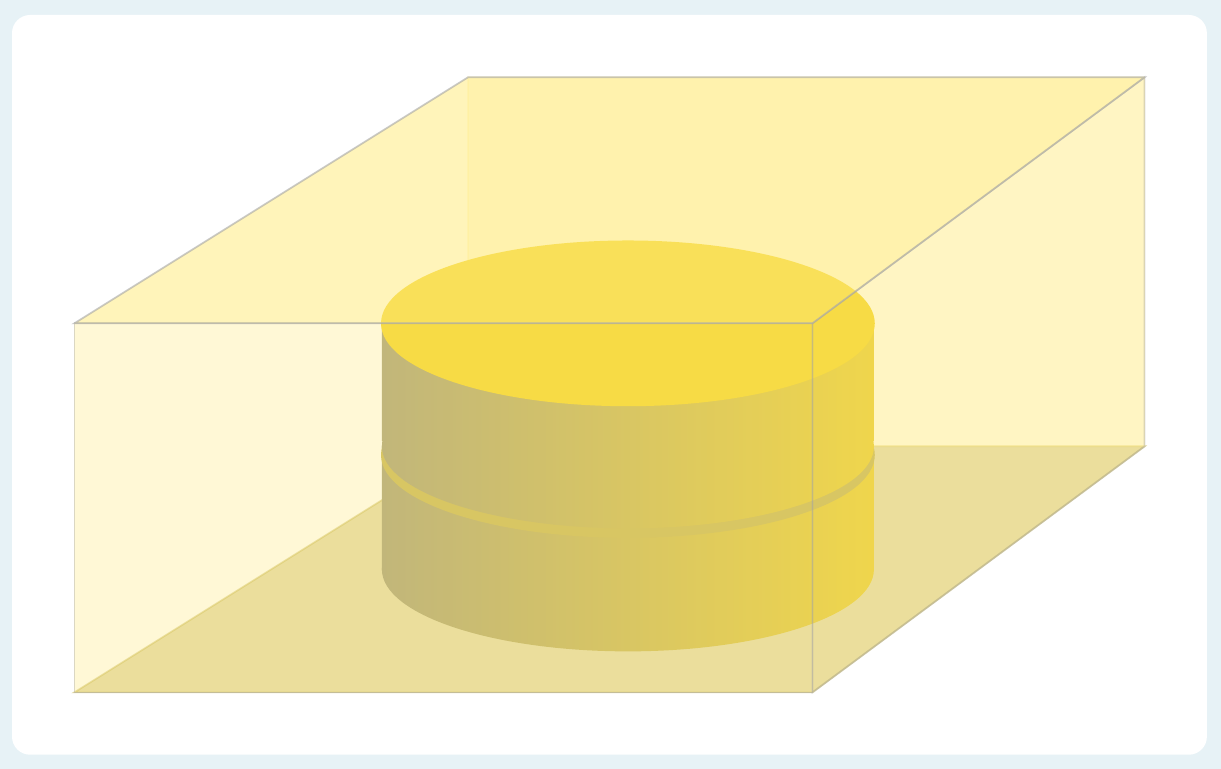
\includegraphics[scale=0.36]{resources/Gold.PNG}}
\subfigure[]{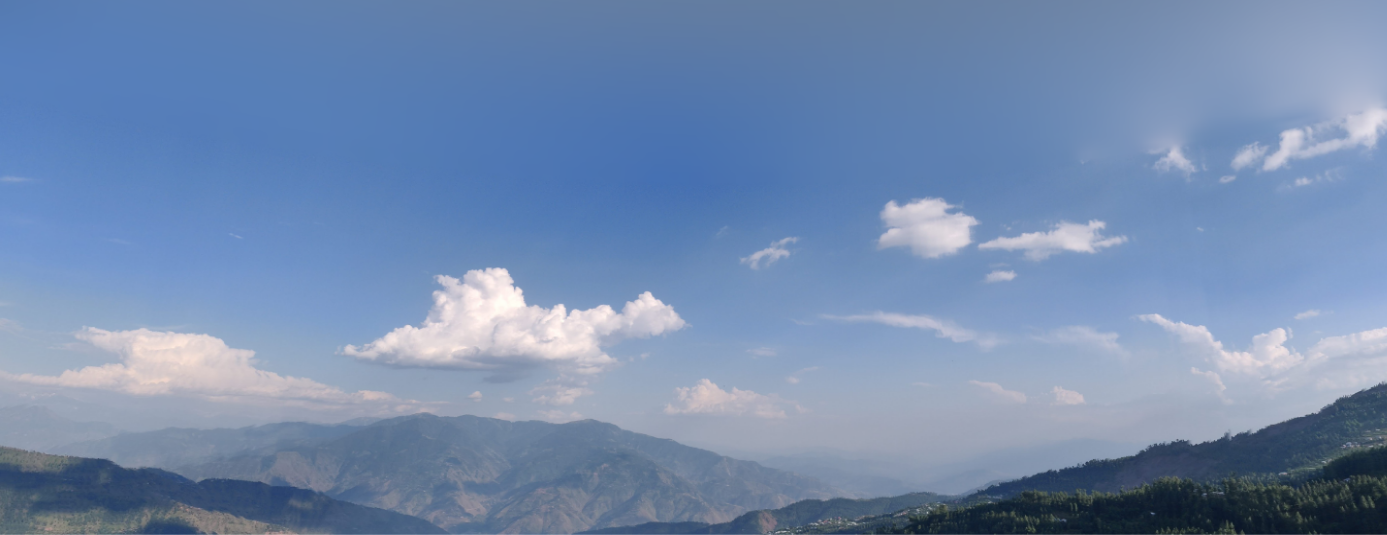
\includegraphics[scale=0.1]{resources/home.png}}
}
}
}
\section{Including Graphics}
\SingleFrame{Including Graphics}{
Graphics environment is based on mini page. You can include as many figures as you can. \\
\alert{$\backslash$Figures\{List of graphics as Subfigures Here\}} \\
For example, the two pictures on previous slide were added as: \\
 \gNode{\alert{$\backslash$Figures\{ \\
	$\backslash$subfigure[]\{$\backslash$includegraphics[scale=0.36]\{resources/Gold.PNG\}\} \\
	$\backslash$subfigure[]\{$\backslash$includegraphics[scale=0.1]\{resources/home.png\}\} \\
	\}} }
\rNode{{\bf \large \alert{This Package is Flexible}} \\
	You can use all defined \LaTeX environments inside frames.}
}
\section{Progress Bar}
\DoubleFrame{Progress Bar}{
\rNode{} \gNode{}
	\kNode{The progress bar in footline shows slide number. You can see that title also changes color when slides progress. \alert{$\backslash$sNode\{Text\}} changes text color slide to slide unless specified otherwise.}
}
{
	\sNode{Progress bar also shows stopwatch over a predefined presentation time by setting \alert{$\backslash$pgfmathsetmacro\{$\backslash$TotalTime\}\{Minutes\}} in permeable of document. Time is shown only in Adobe Reader. The package \alert{tdclock} from CTAN is used to fetch system time in document.}
}
%-----------------------------------------------------------------------
%	PRESENTATION SLIDE FINAL
%-----------------------------------------------------------------------
{
\usebackgroundtemplate{\begin{tikzpicture}
	\node[align=center,opacity=0.7]{ 
\includegraphics[width=0.55\paperwidth]{resources/ud.png}};
	\end{tikzpicture}}
\begin{frame}[plain,noframenumbering]
\vfill \hfill
	
\begin{tikzpicture}
	\draw[] node[align=center, text width=0.4\textwidth,inner sep=10pt,opacity=0.6] {{\color{blue!70!green} \bf \LARGE THANKS } \\ \qquad \\
\href{https://github.com/massgh/Beamer-Timer/tree/master/}{\bf \color{blue!80!black}Beamer-Timer@Github}\\ \qquad \\
	\href{https://github.com/massgh/Vasp2Visual/tree/master/}{\bf \color{blue!80!black}Vasp2Visual@Github}		
};
\end{tikzpicture}
\end{frame}
}
\end{document}
